\section{DONANIM BİLEŞENLERİ VE BAĞLANTI ŞEMALARI}

Bu bölümde, sistemde kullanılan tüm donanım bileşenleri, teknik özellikleri ve Arduino Uno'ya bağlantı detayları açıklanmaktadır.

\subsection{Arduino Uno}

Arduino Uno, ATmega328P mikrodenetleyicisine dayanan açık kaynaklı bir geliştirme kartıdır. 16~MHz kristal osilatör ile çalışır, 32~KB flash program belleğine, 2~KB SRAM'e ve 1~KB EEPROM'a sahiptir. 14 dijital giriş/çıkış pini (6 tanesi PWM destekli) ve 6 analog giriş pini bulunmaktadır. Bu projede Arduino Uno, tüm alt sistemlerin merkezi denetleyicisi olarak görev yapmaktadır.

\begin{table}[H]
    \centering
    \small
    \renewcommand{\arraystretch}{0.9}
    \caption{Arduino Uno pin atamaları}
    \label{tab:pin_atama}
    \begin{tabular}{|l|l|l|}
        \hline
        \textbf{Pin} & \textbf{Bileşen} & \textbf{Açıklama} \\
        \hline
        D2 & Buton & Radar aç/kapat (GND arası) \\
        \hline
        D4 & SD Kart CS & SPI chip select \\
        \hline
        D6 & Tilt Servo & SG90S sinyal pini \\
        \hline
        D9 & Pan Servo & MG90S sinyal pini \\
        \hline
        D10 & SPI SS & SPI slave select (çıkış) \\
        \hline
        D11 & SD Kart MOSI & SPI veri çıkışı \\
        \hline
        D12 & SD Kart MISO & SPI veri girişi \\
        \hline
        D13 & SD Kart SCK & SPI saat sinyali \\
        \hline
        A0 & Sharp Sensör & Analog mesafe çıkışı \\
        \hline
        A4 & I2C SDA & MPU6050 ve LCD veri \\
        \hline
        A5 & I2C SCL & MPU6050 ve LCD saat \\
        \hline
    \end{tabular}
\end{table}

\subsection{Sharp GP2Y0A02YK0F Kızılötesi Mesafe Sensörü}

Sharp GP2Y0A02YK0F \cite{sharp_datasheet}, kızılötesi ışık yayan bir LED ve pozisyon duyarlı bir dedektörden (PSD) oluşan aktif bir mesafe algılama sensörüdür. 20--150~cm aralığında analog çıkış gerilimi üretir. Sensör, üçgenleme (triangulation) prensibi ile çalışmaktadır: yayılan IR ışın hedeften yansıyarak PSD üzerine düşer ve ışının düşme noktası mesafeye bağlı olarak değişir.

\begin{figure}[H]
\centering
	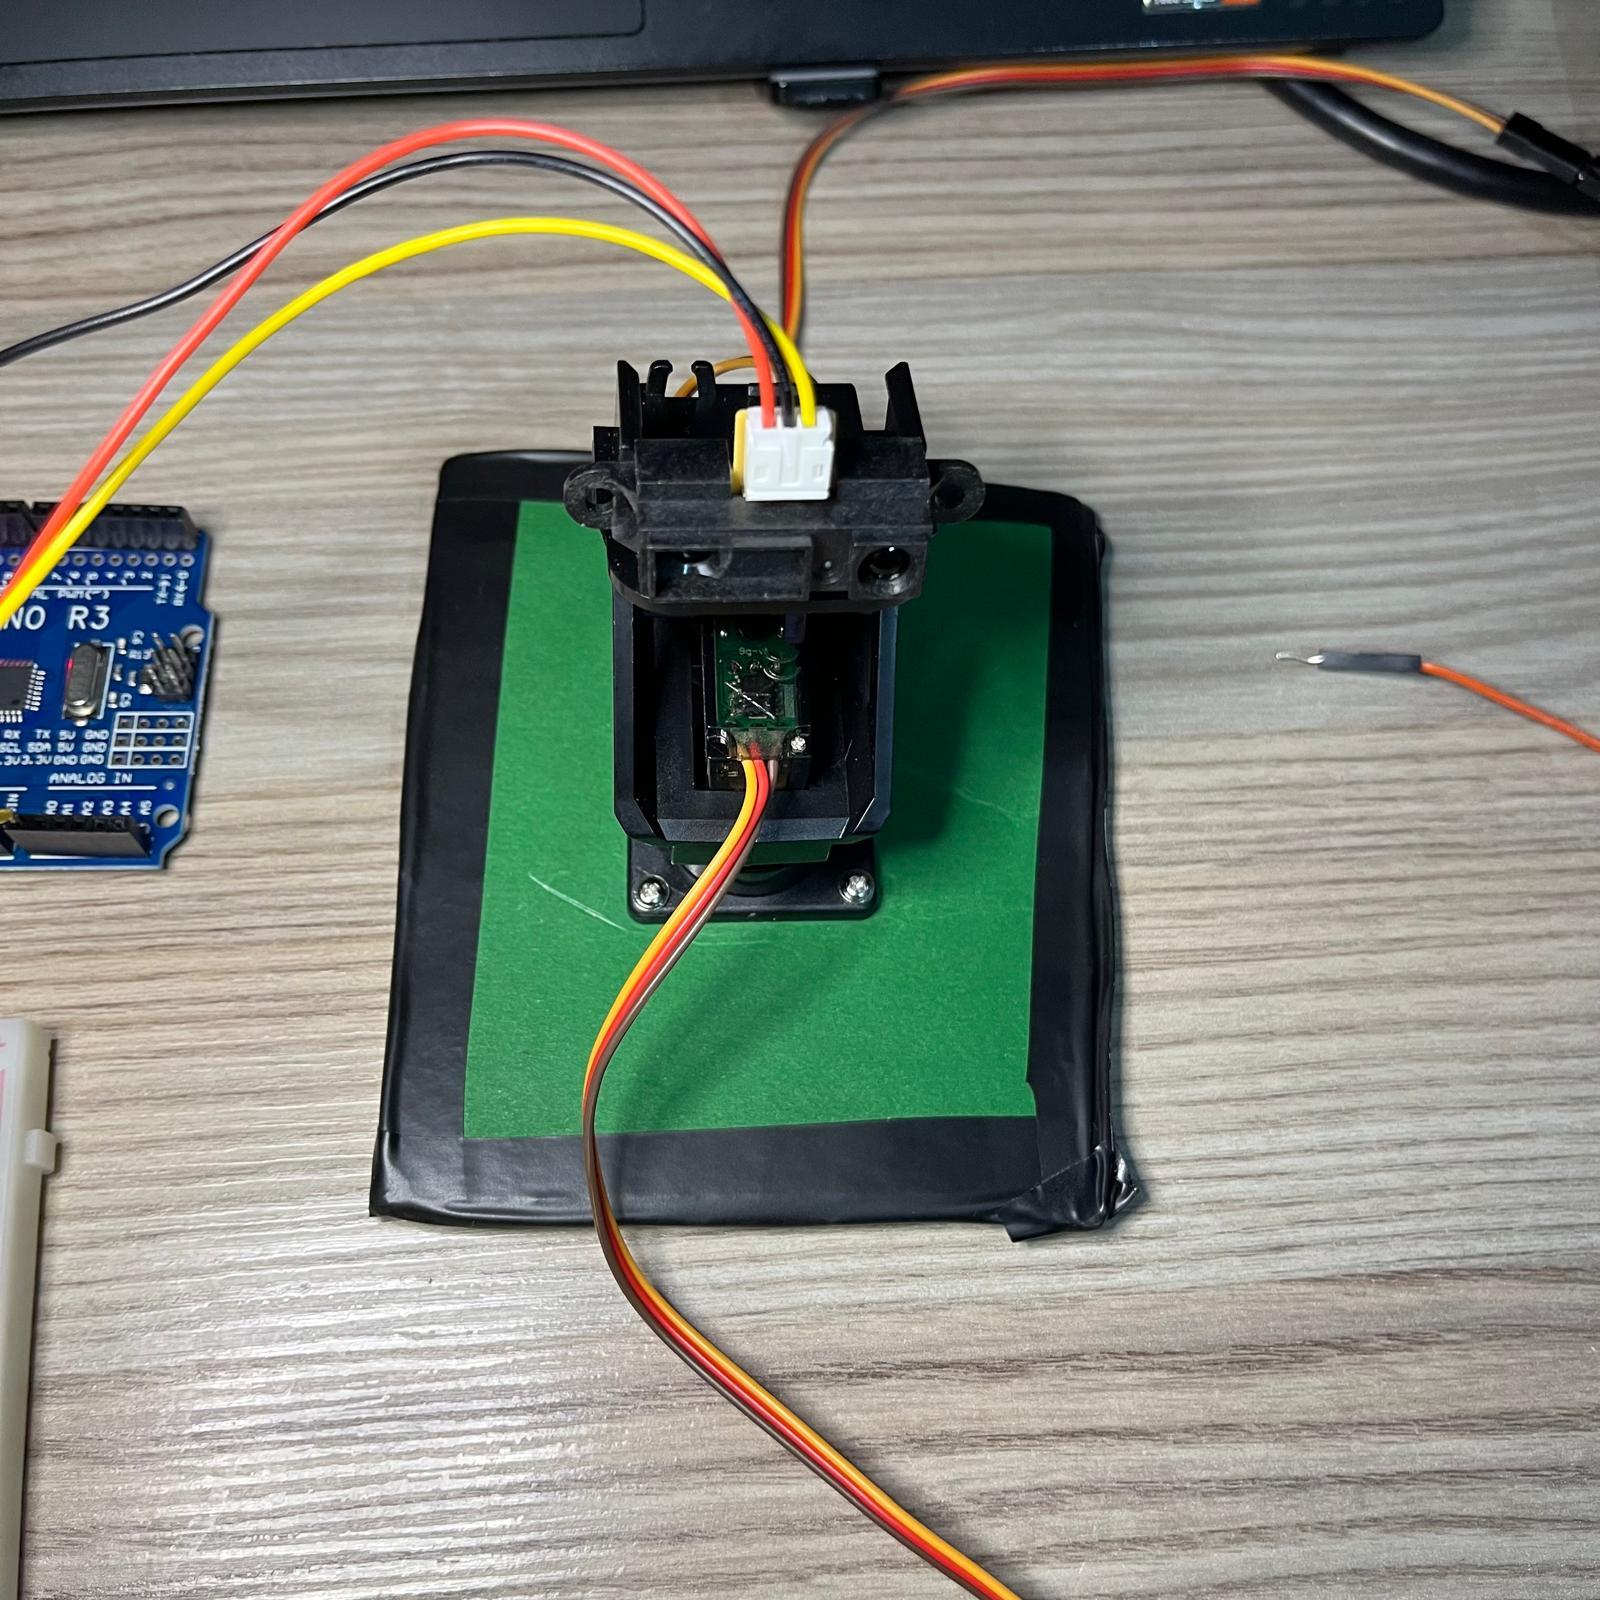
\includegraphics[width=0.5\textwidth]{sharp_sensor.jpeg}
	\caption{Sharp GP2Y0A02YK0F kızılötesi mesafe sensörü}
    \label{fig:sharp_sensor}
\end{figure}

Sensörün gövde yapısı ve bağlantı uçları Şekil~\ref{fig:sharp_yapi}'de gösterilmektedir. Bu görsel, sensörün Vcc, GND ve analog çıkış bağlantılarının ayırt edilmesi için kullanılmıştır.

\begin{figure}[H]
\centering
	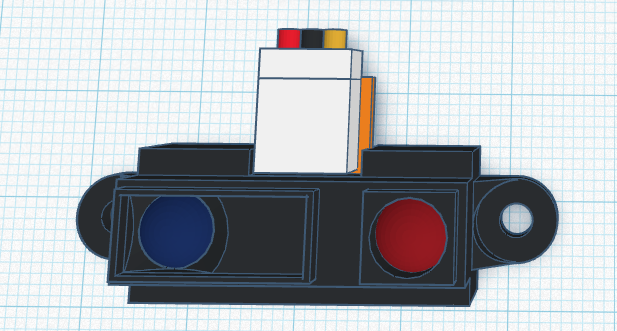
\includegraphics[width=0.5\textwidth]{sharp.png}
	\caption{Sharp GP2Y0A02YK0F sensör gövdesi ve pin yapısı}
    \label{fig:sharp_yapi}
\end{figure}

Sensörün Arduino'ya bağlantısı Şekil~\ref{fig:sharp_baglanti}'de gösterilmektedir. Sensörün Vo (çıkış) pini A0 analog giriş pinine, Vcc pini 5V'a ve GND pini toprak hattına bağlanmaktadır.

\begin{figure}[H]
\centering
	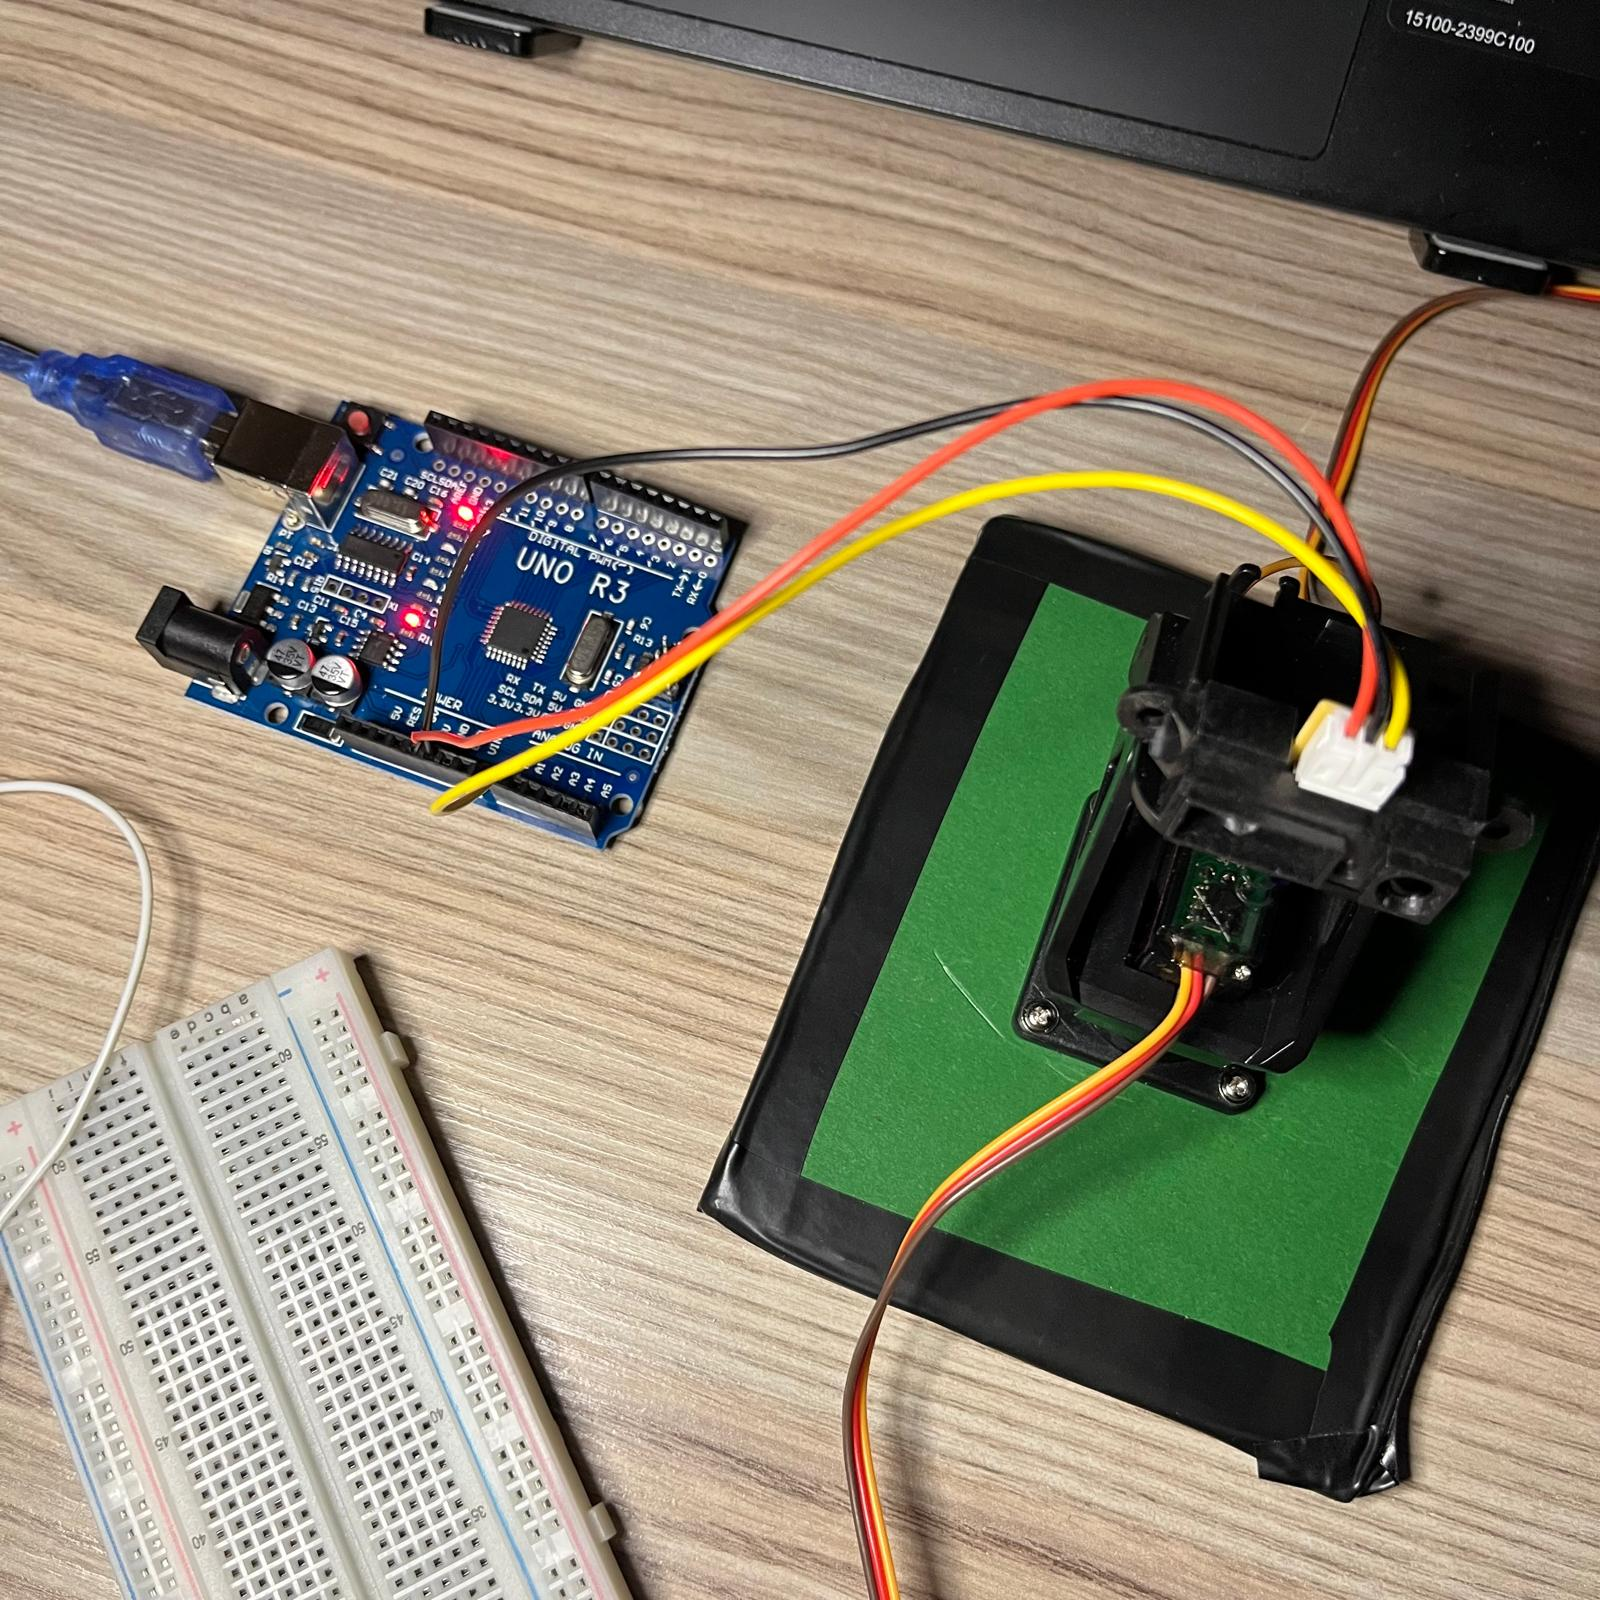
\includegraphics[width=0.65\textwidth]{sharp_baglanti.jpeg}
	\caption{Sharp sensör bağlantı şeması}
    \label{fig:sharp_baglanti}
\end{figure}

\subsection{Servo Motorlar}

Projede iki adet servo motor kullanılmaktadır:

\begin{itemize}
    \item \textbf{MG90S (Pan servo):} Metal dişli yapısıyla daha yüksek tork sağlar. Yatay eksen taraması için D9 pinine bağlıdır. 20--160 derece aralığında çalıştırılmaktadır.
    \item \textbf{SG90S (Tilt servo):} Plastik dişli, hafif yapılı servo motor. Dikey eksen hareketi için D6 pinine bağlıdır. 84--96 derece arasında küçük açılarla gezdirilmektedir.
\end{itemize}

Servo motorlar PWM sinyali ile kontrol edilir. Her servo için üç kablo bulunur: sinyal (sarı/turuncu), Vcc (kırmızı) ve GND (kahverengi). Servo motorların Arduino'nun 5V pininden beslenmesi önerilmez; ani akım çekimi Arduino'nun reset atmasına yol açabilir. Bu nedenle servo motorlar için harici bir güç kaynağı (4'lü pil yatağı, yaklaşık 6V) kullanılması tavsiye edilmektedir. Harici güç kaynağı kullanıldığında GND hatlarının ortak bağlanması zorunludur.

\begin{figure}[H]
\centering
	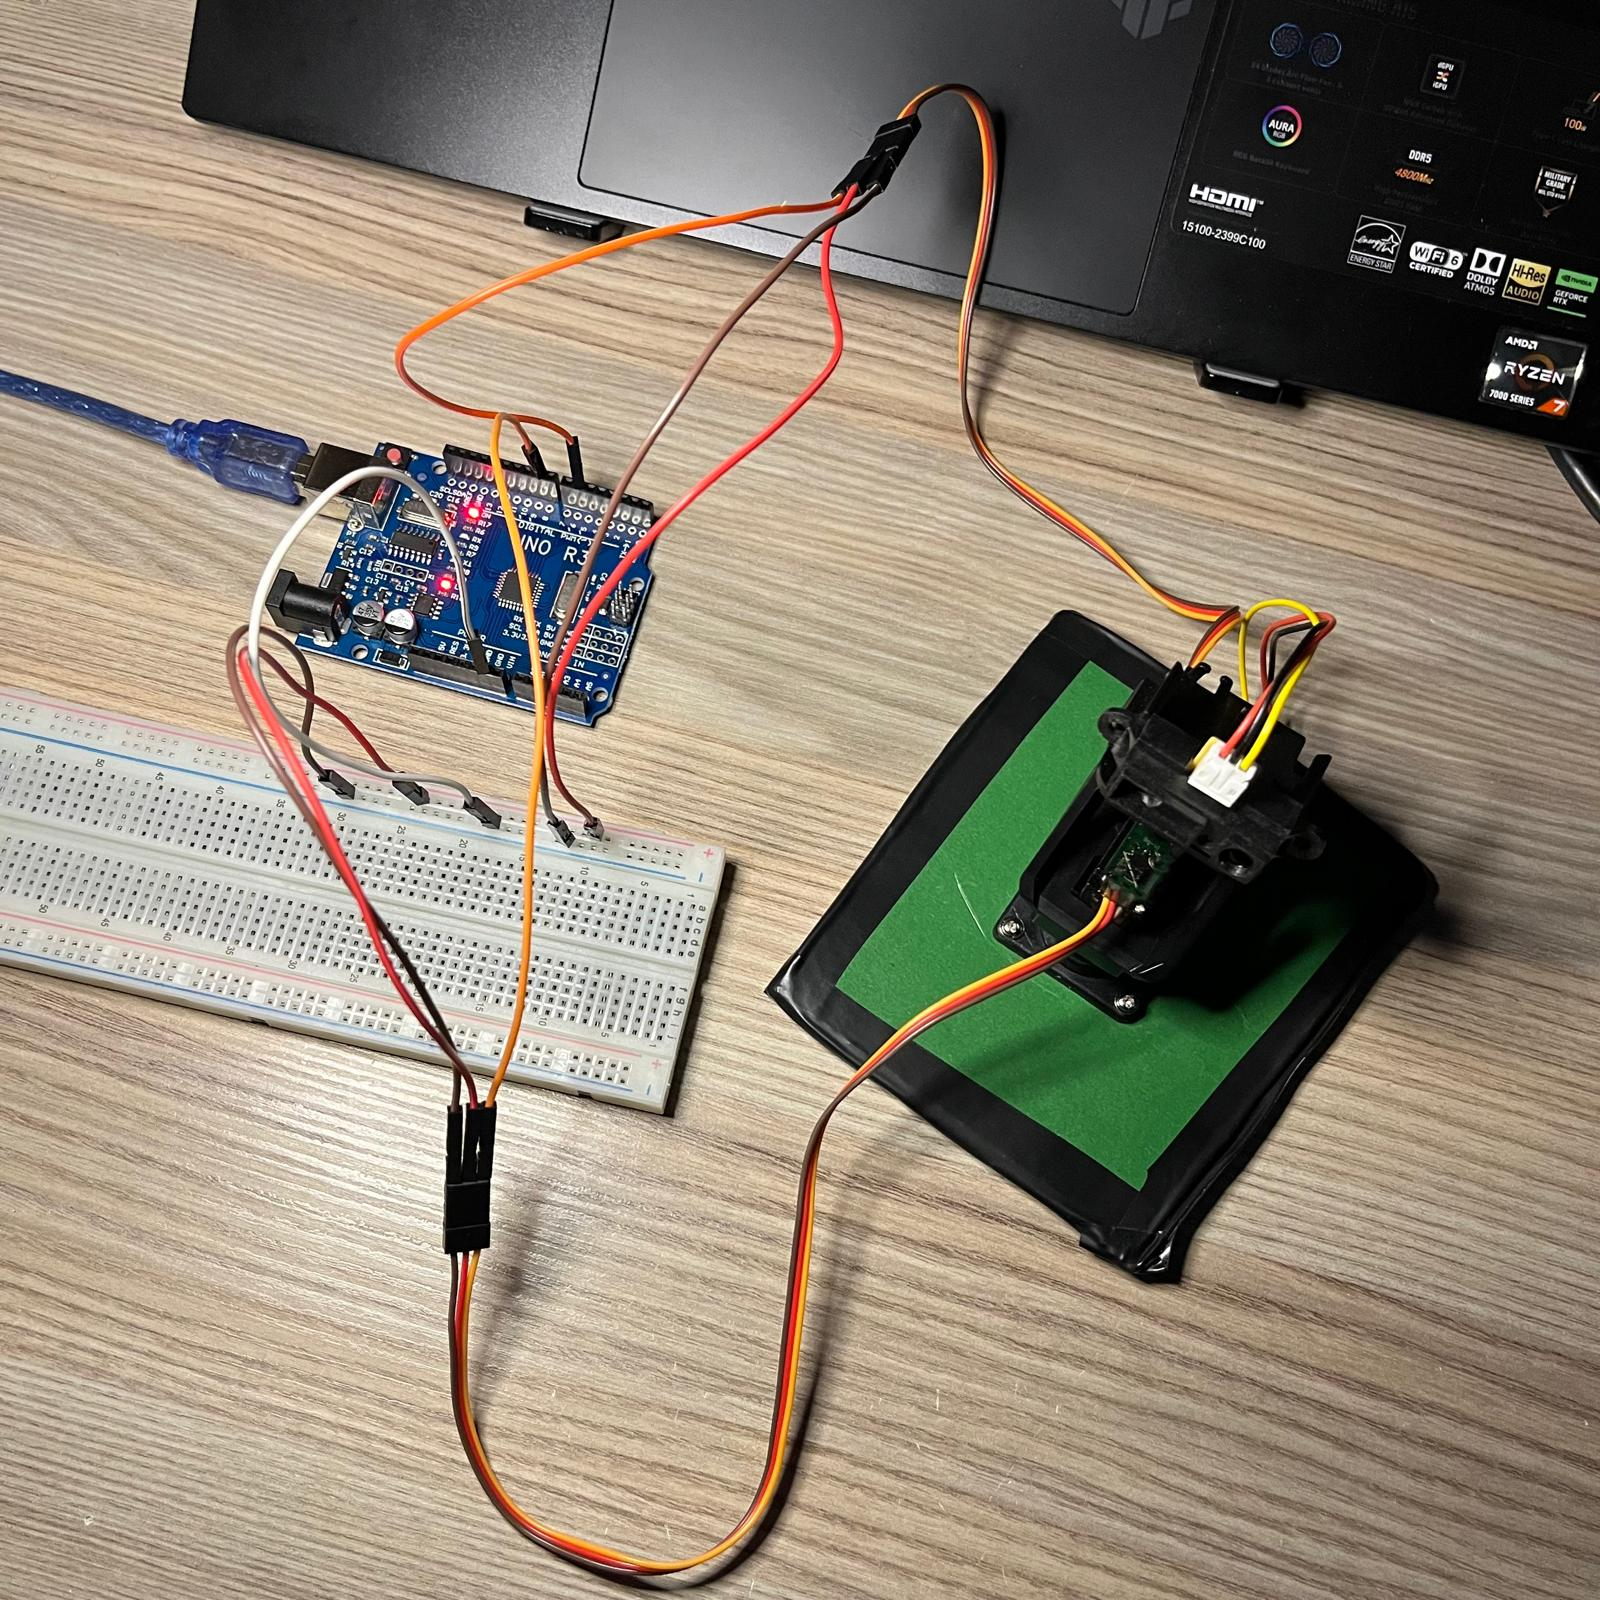
\includegraphics[width=0.65\textwidth]{servo_baglanti.jpeg}
	\caption{Servo motor bağlantı şeması}
    \label{fig:servo_baglanti}
\end{figure}

\begin{figure}[H]
\centering
	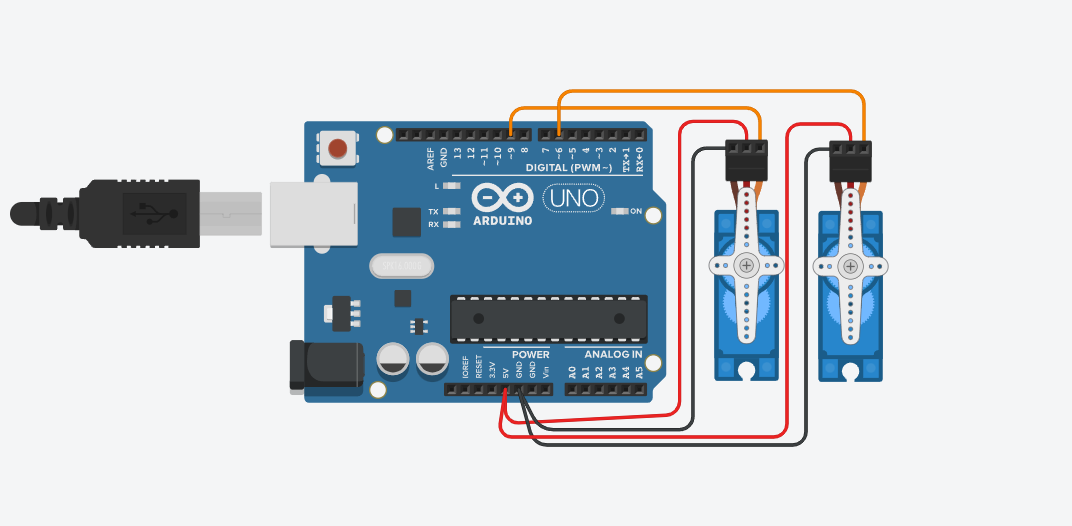
\includegraphics[width=0.55\textwidth]{servo_baglanti.png}
	\caption{Servo motor sinyal bağlantı detayı}
    \label{fig:servo_baglanti_detay}
\end{figure}

\subsection{Pan-Tilt Mekanizma}

Pan-tilt mekanizma, iki servo motorun birbirine dik açıda monte edilmesiyle oluşturulmuş iki serbestlik dereceli bir hareket platformudur. Pan servo altta sabit gövdeye monte edilir ve yatay dönüşü sağlar. Tilt servo, pan servo üzerine monte edilir ve dikey eğim hareketini gerçekleştirir. Sharp sensör, tilt servonun ucuna bağlanarak tarama yönünü takip eder.

\begin{figure}[H]
\centering
\begin{subfigure}[b]{0.45\textwidth}
    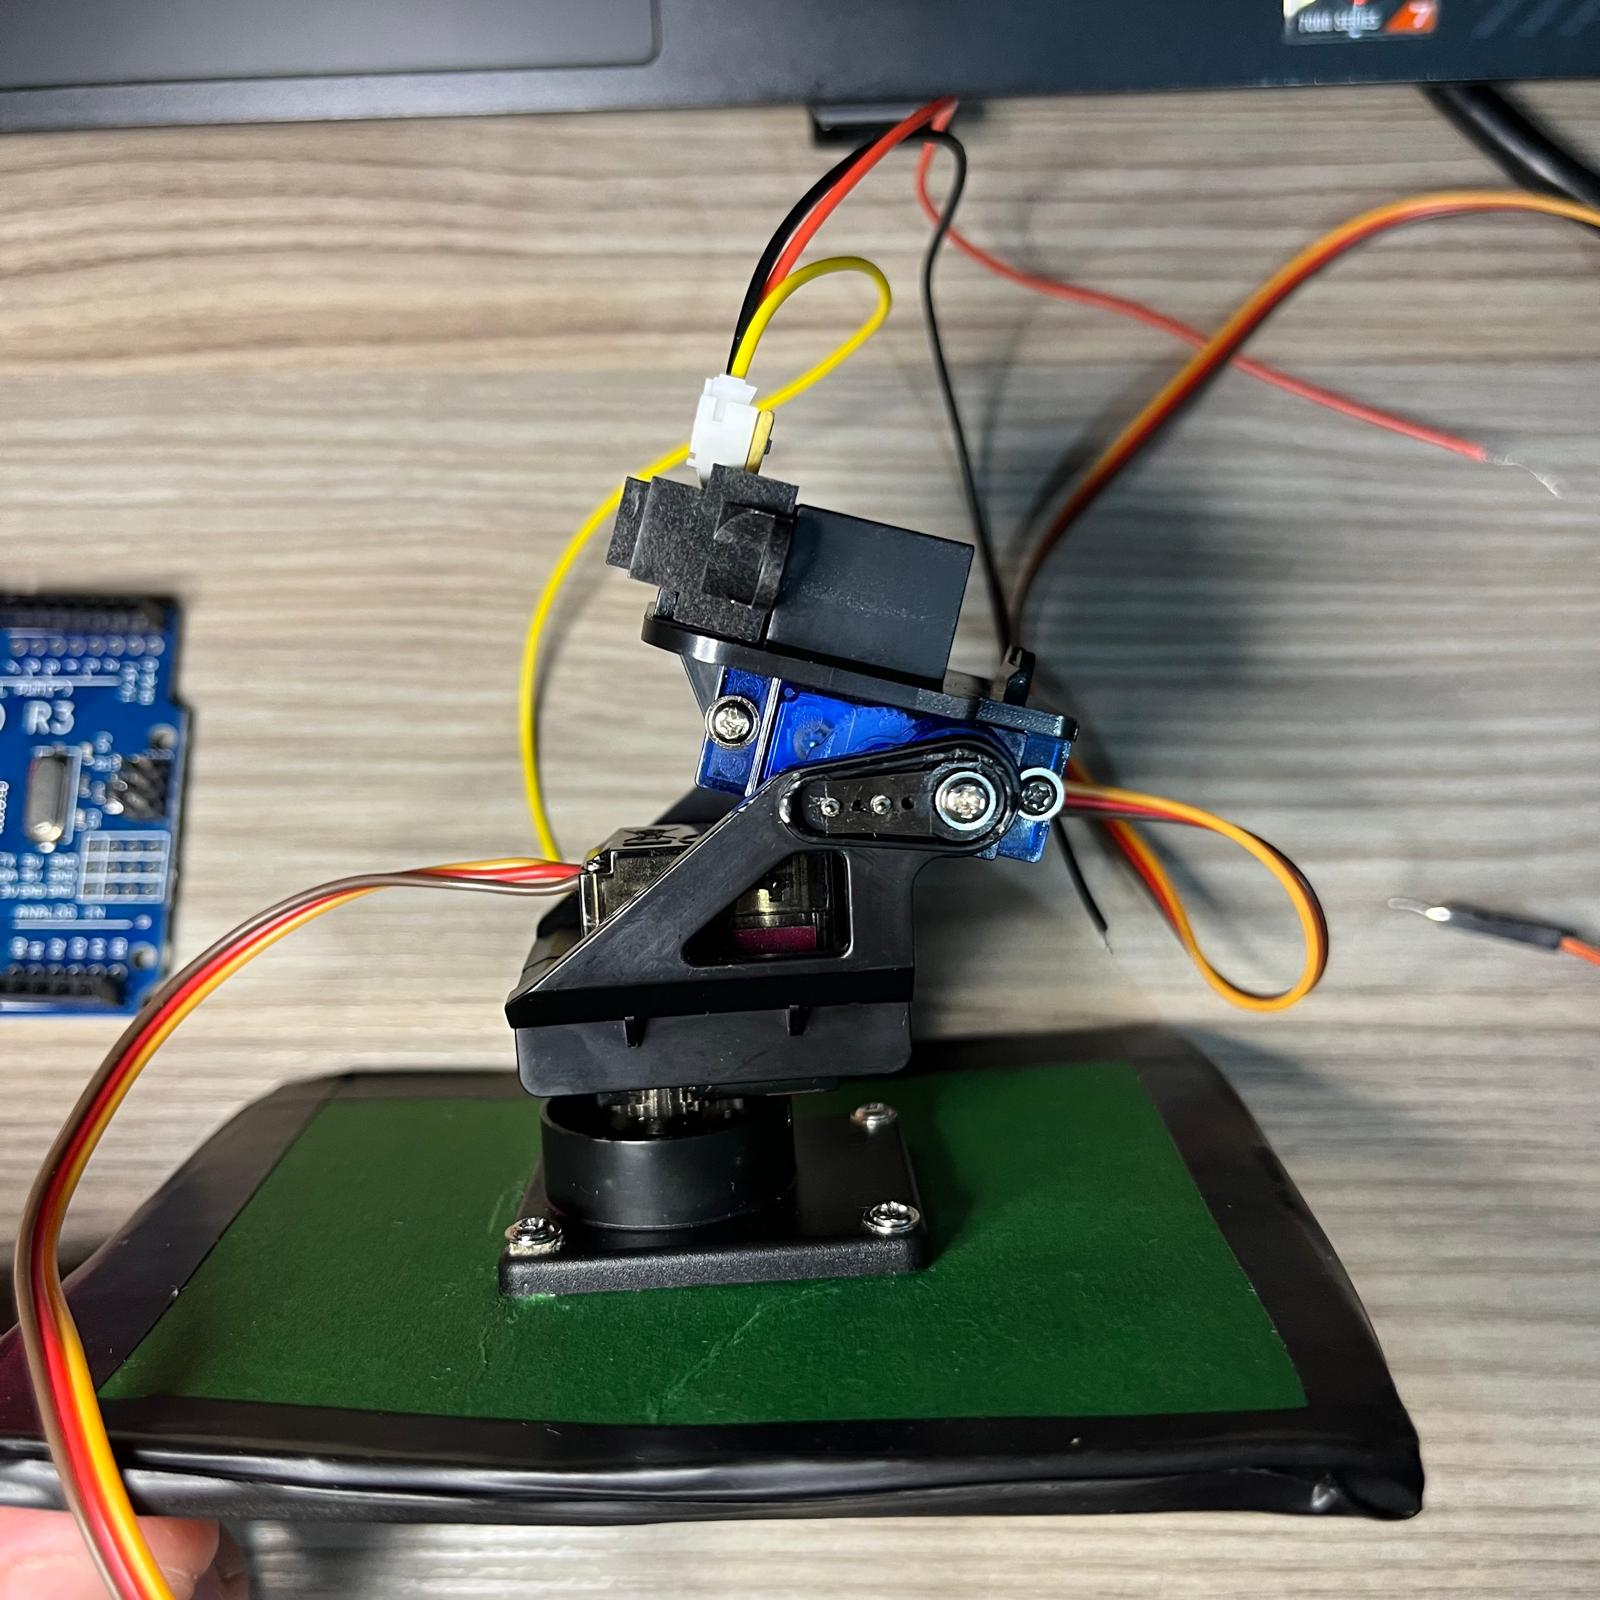
\includegraphics[width=\textwidth]{pan_titl_mek1.jpeg}
    \caption{Pan-tilt mekanizma -- ön/yandan görünüm}
\end{subfigure}
\hfill
\begin{subfigure}[b]{0.45\textwidth}
    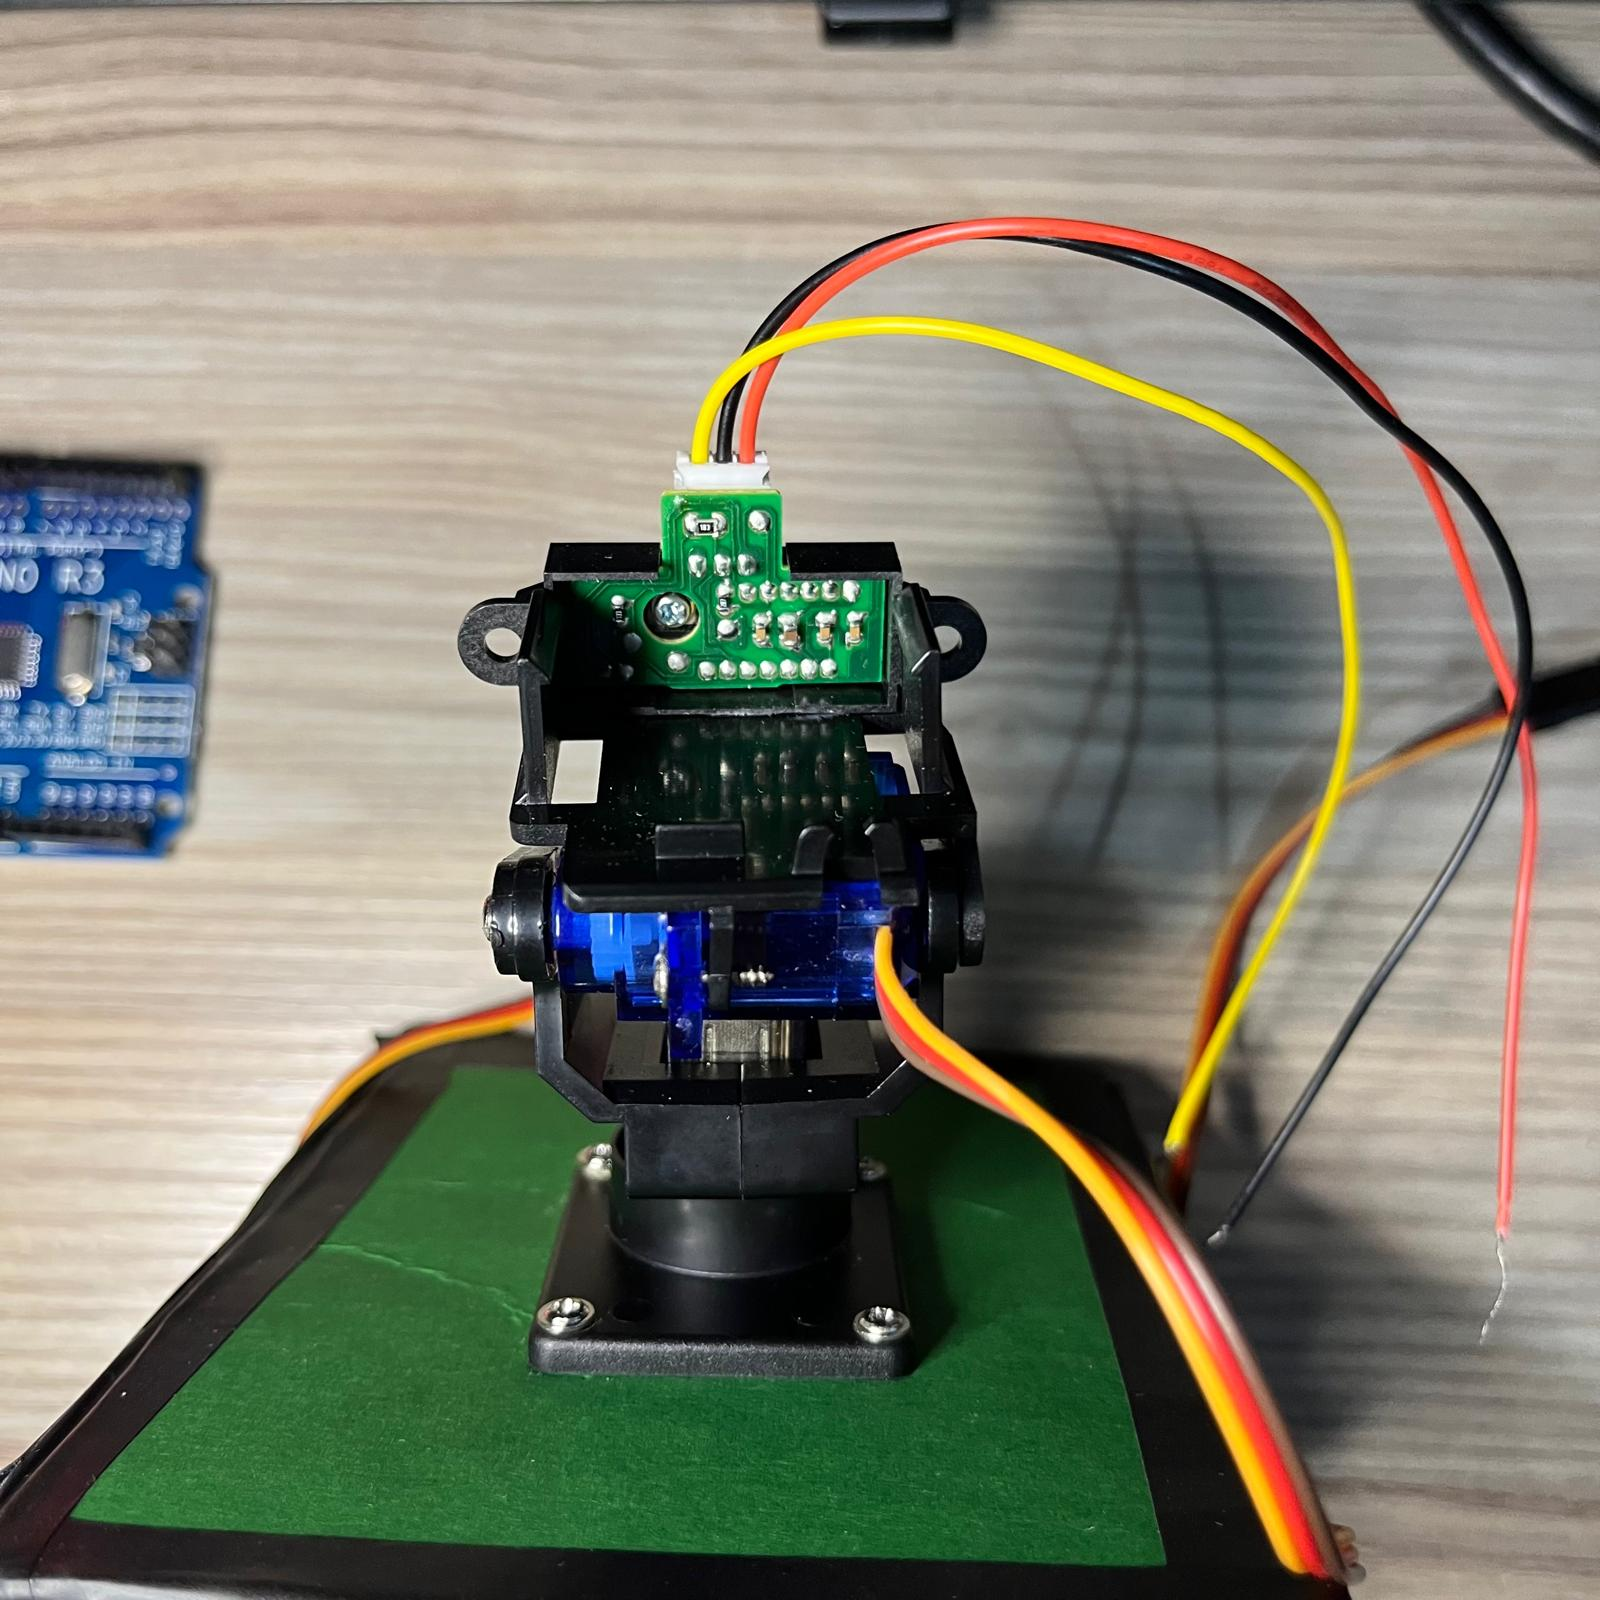
\includegraphics[width=\textwidth]{pan_tilt_mek2.jpeg}
    \caption{Pan-tilt mekanizma -- sensör bağlantı görünümü}
\end{subfigure}
\caption{Pan-tilt mekanizma fotoğrafları}
\label{fig:pan_tilt_mek}
\end{figure}

\subsection{MPU6050 İvmeölçer/Jiroskop Modülü}

MPU6050 \cite{mpu6050_datasheet}, InvenSense (şimdi TDK) tarafından üretilen 6 eksenli bir ataletsel ölçüm birimi (IMU) modülüdür. 3 eksen ivmeölçer ($\pm 2g$, $\pm 4g$, $\pm 8g$, $\pm 16g$) ve 3 eksen jiroskop ($\pm 250$, $\pm 500$, $\pm 1000$, $\pm 2000$ derece/saniye) içermektedir. Bu projede $\pm 2g$ ve $\pm 250$ derece/saniye hassasiyet aralıkları seçilmiştir.

\begin{figure}[H]
\centering
	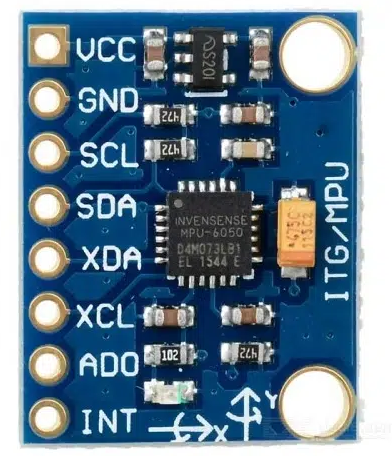
\includegraphics[width=0.35\textwidth]{mpu.png}
	\caption{MPU6050 modülü}
    \label{fig:mpu}
\end{figure}

Modül I2C protokolü üzerinden 0x68 adresinde haberleşmektedir. Bağlantı detayları Şekil~\ref{fig:mpu_baglanti}'de gösterilmektedir.

\begin{figure}[H]
\centering
	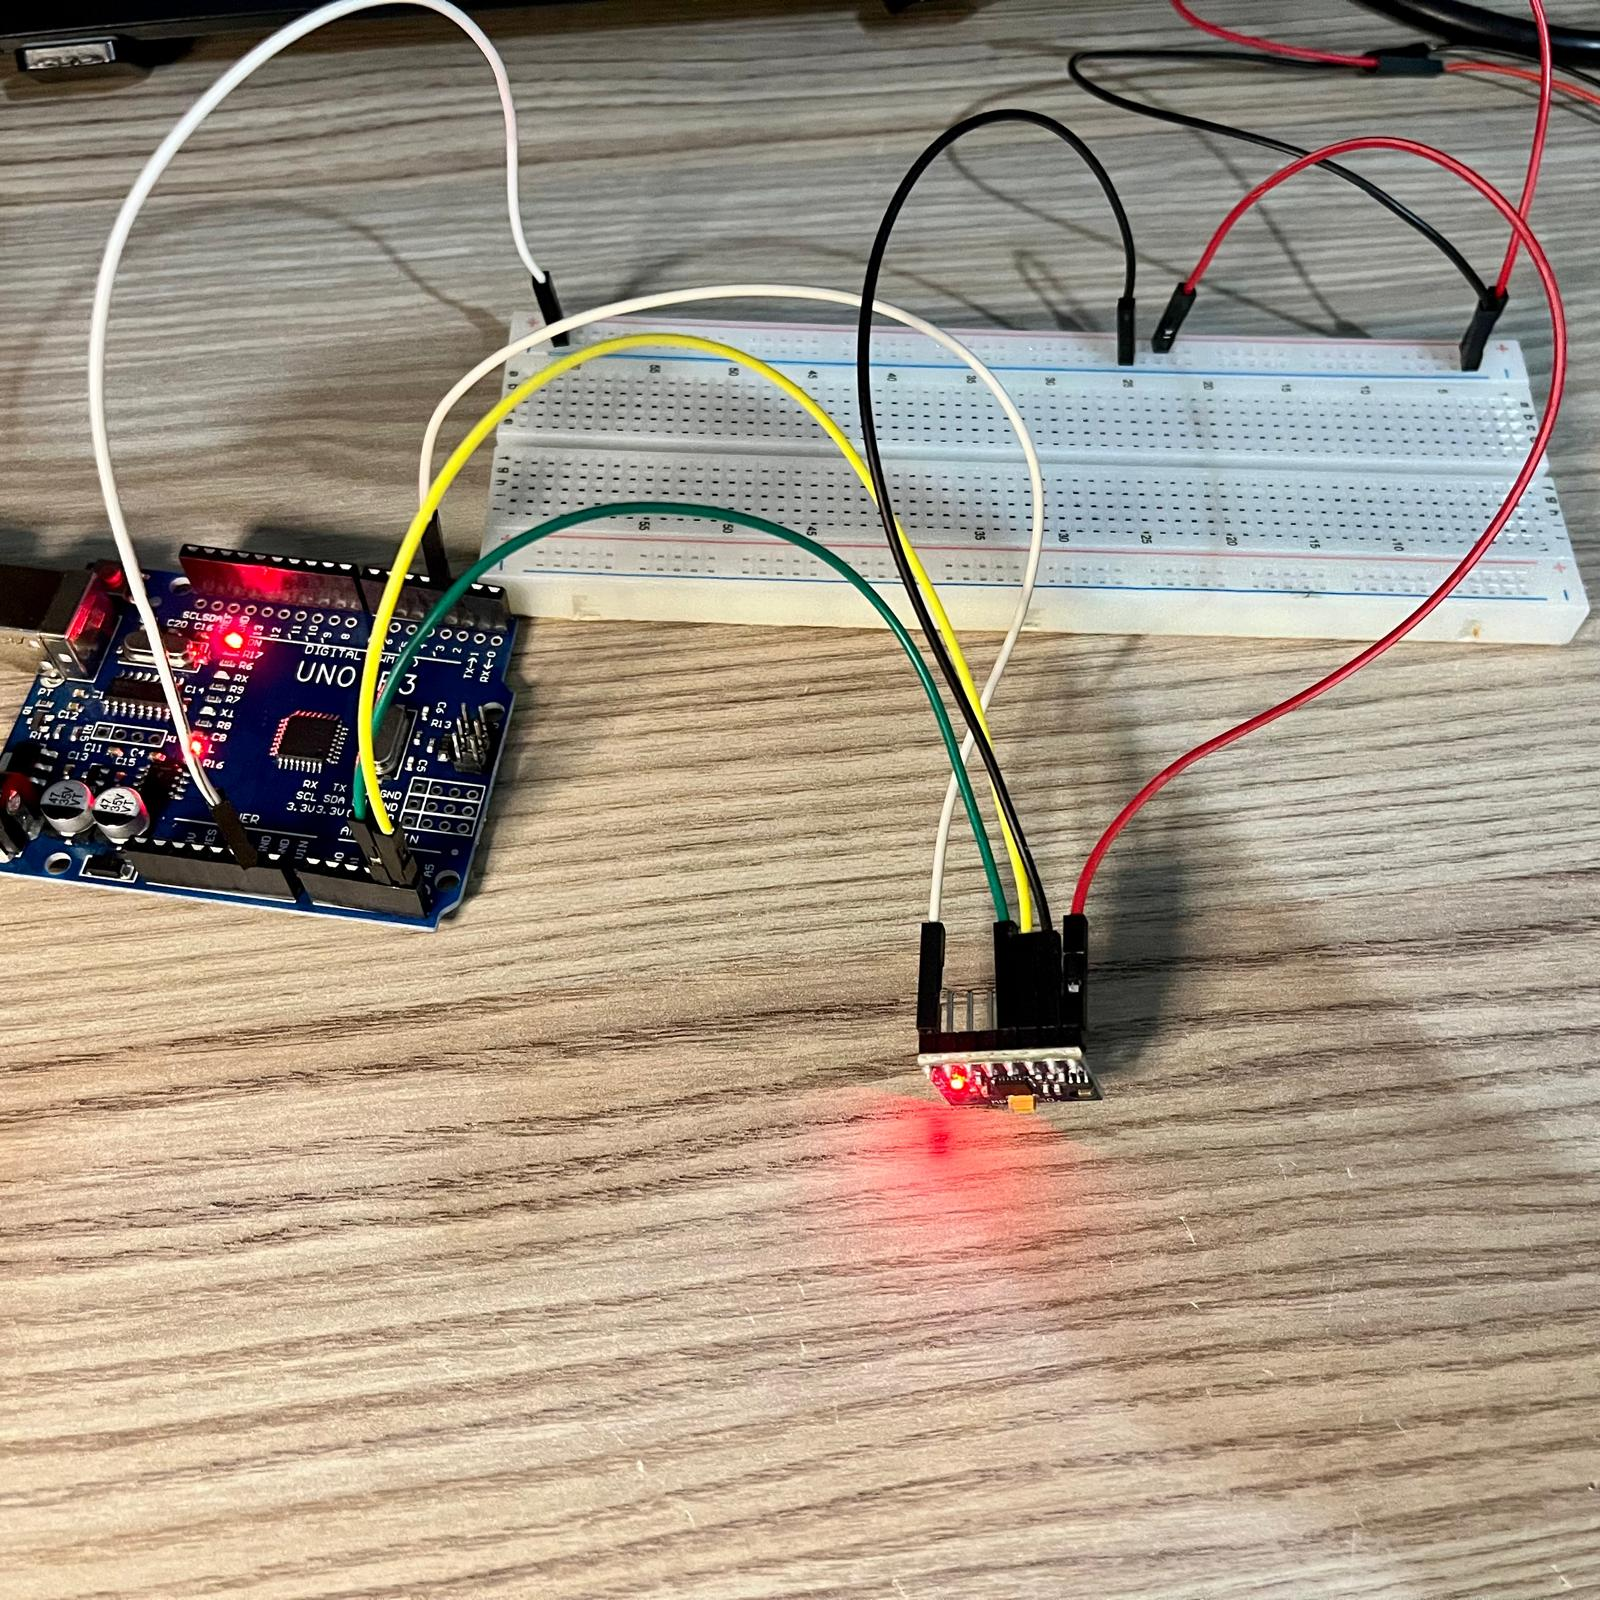
\includegraphics[width=0.55\textwidth]{mpu_baglanti.jpeg}
	\caption{MPU6050 bağlantı şeması}
    \label{fig:mpu_baglanti}
\end{figure}

\subsection{SD Kart Modülü}

SPI arayüzlü SD kart modülü, tarama verilerinin kalıcı olarak kaydedilmesi amacıyla kullanılmaktadır. Modül, micro SD kartları desteklemekte olup FAT16, FAT32 ve exFAT dosya sistemleri ile çalışabilmektedir. SPI bağlantısında CS pini D4'e atanmıştır.

\begin{figure}[H]
\centering
	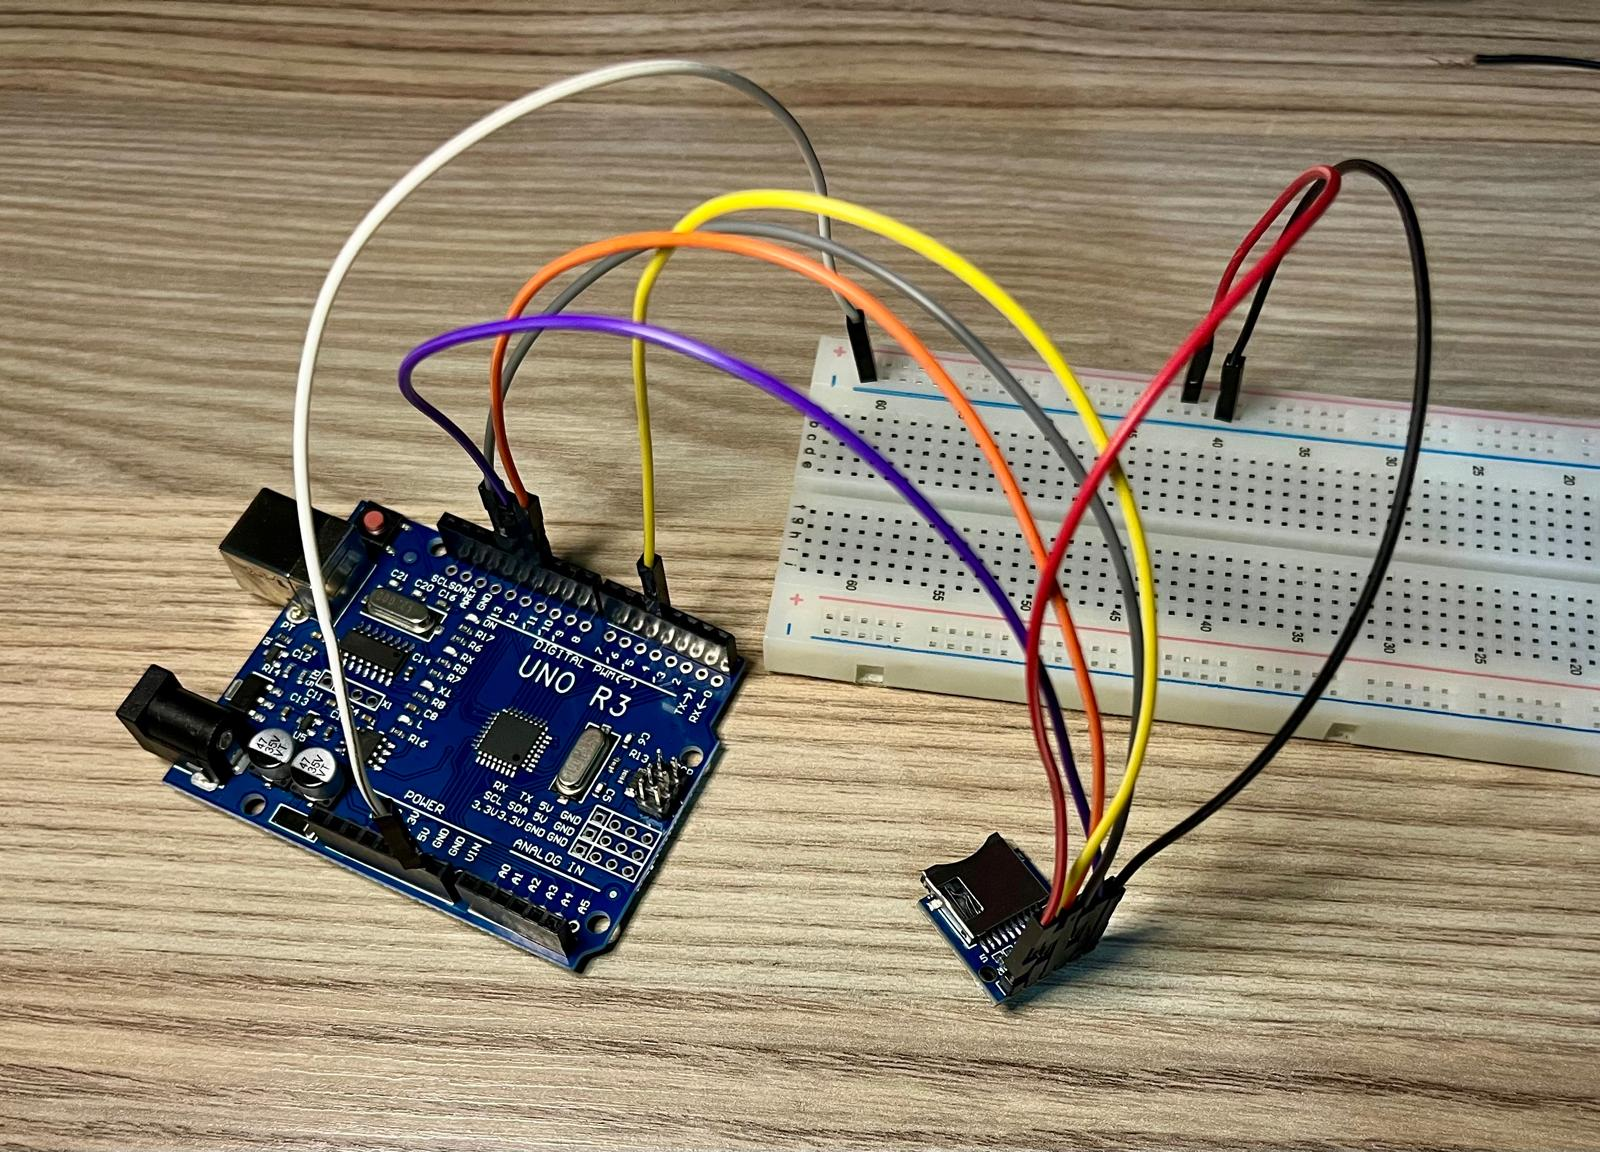
\includegraphics[width=0.55\textwidth]{spi_sd_kart_baglanti.jpeg}
	\caption{SD kart modülü SPI bağlantı şeması}
    \label{fig:sd_baglanti}
\end{figure}

\subsection{16x2 I2C LCD Ekran}

16 sütun ve 2 satırdan oluşan karakter LCD ekran, PCF8574 tabanlı I2C arabirim kartı ile Arduino'ya bağlanmıştır. I2C adresi 0x3F olarak yapılandırılmıştır. Ekran, kullanıcıya radar durumu, hedef bilgisi ve ölçüm değerlerini göstermektedir.

\begin{figure}[H]
\centering
	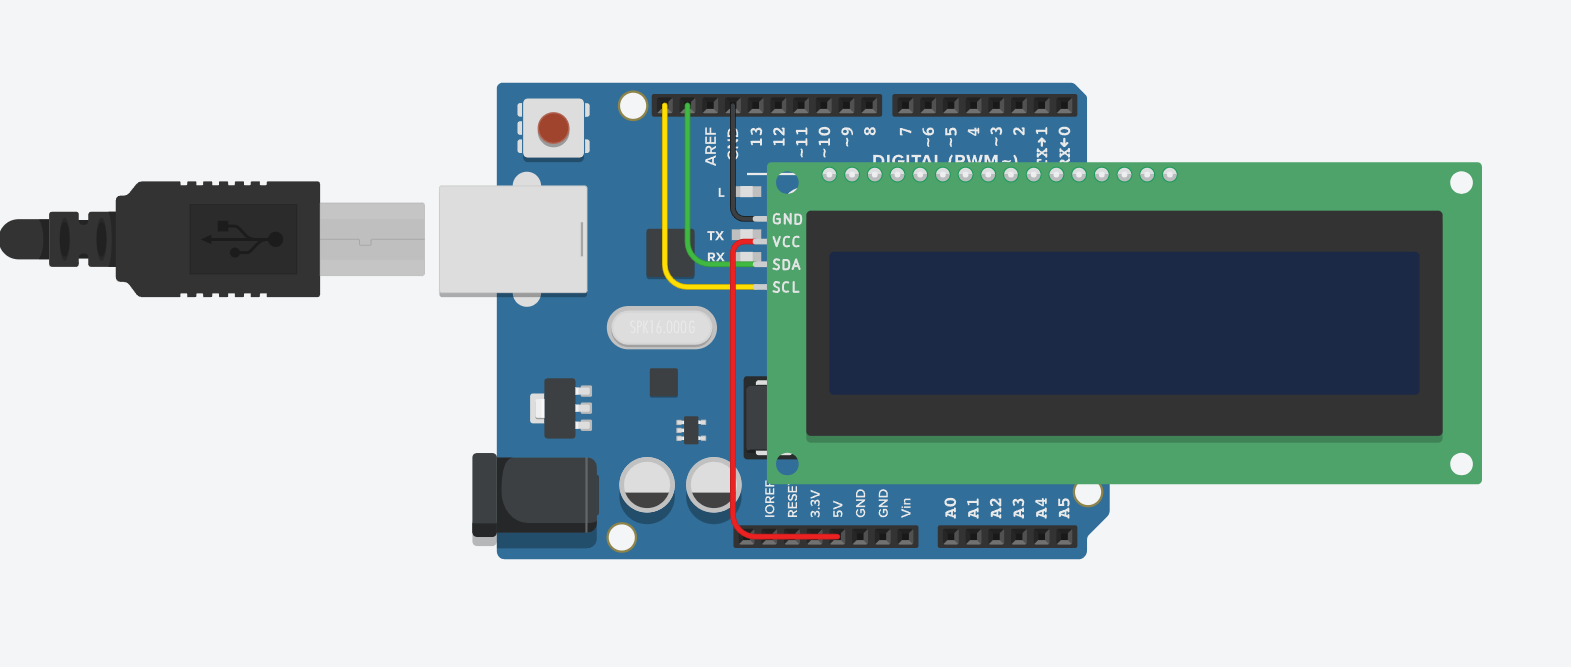
\includegraphics[width=0.55\textwidth]{i2c_baglanti.png}
	\caption{I2C LCD bağlantı pin şeması}
    \label{fig:i2c_lcd_pin}
\end{figure}

\begin{figure}[H]
\centering
	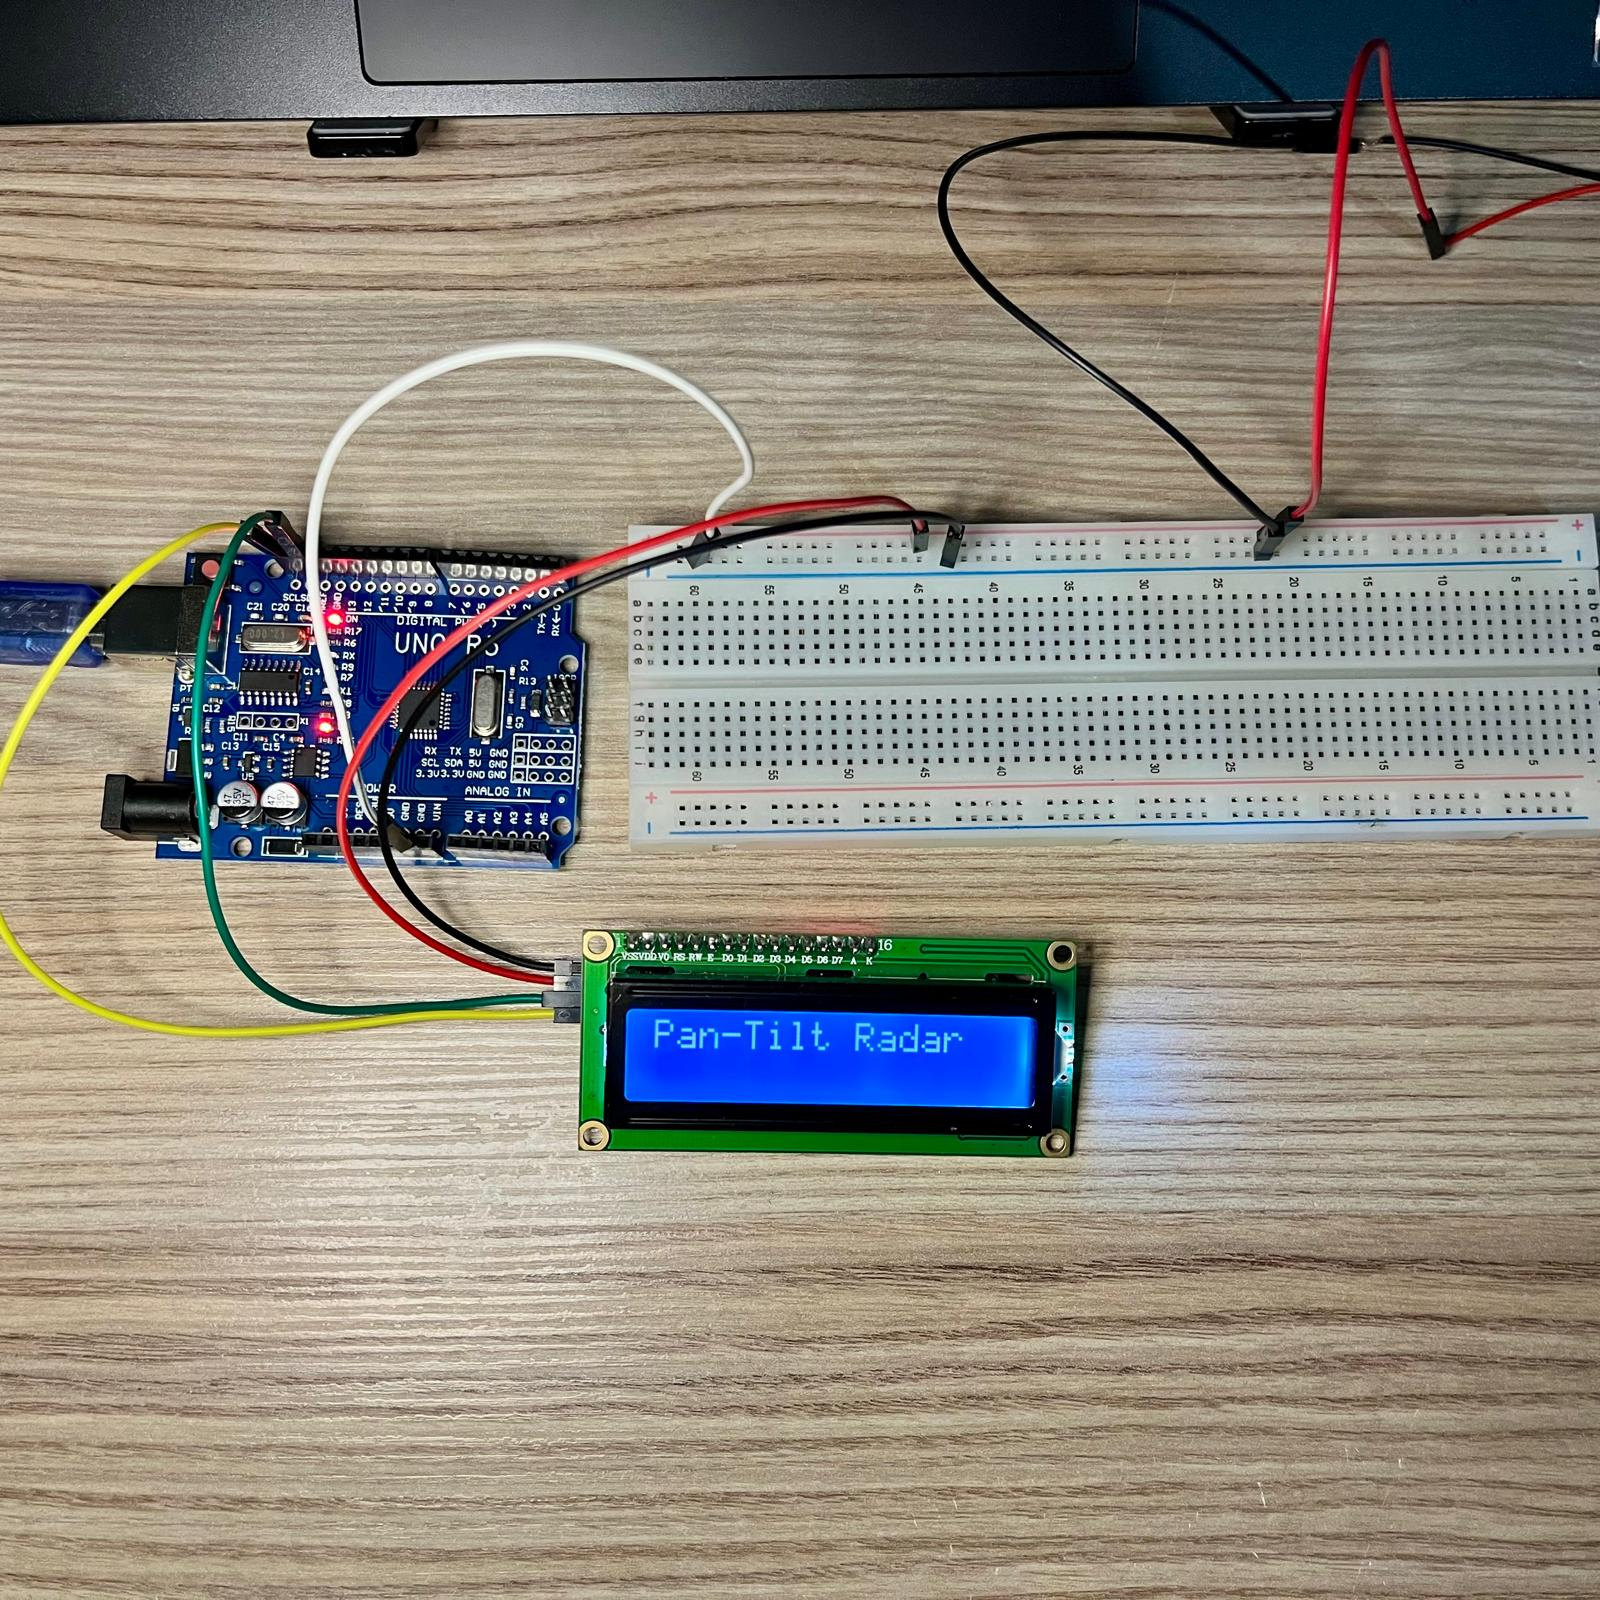
\includegraphics[width=0.55\textwidth]{i2c_baglanti.jpeg}
	\caption{I2C LCD bağlantı devre şeması}
    \label{fig:i2c_lcd_devre}
\end{figure}

\subsection{Güç Besleme}

Sistemin güç beslemesi için iki yaklaşım mevcuttur:

\begin{itemize}
    \item \textbf{USB besleme:} Arduino'nun USB portu üzerinden 5V besleme sağlanır. Servo motorların toplam akım çekimi sınırlı tutulmalıdır.
    \item \textbf{Harici besleme:} 4'lü AA pil yatağı ($\sim$6V) ile servo motorlar doğrudan beslenir. Bu durumda pil yatağının GND hattı Arduino GND ile ortak bağlanmalıdır.
\end{itemize}

Şekil~\ref{fig:guc}'te güç bağlantı şeması gösterilmektedir.

\begin{figure}[H]
\centering
	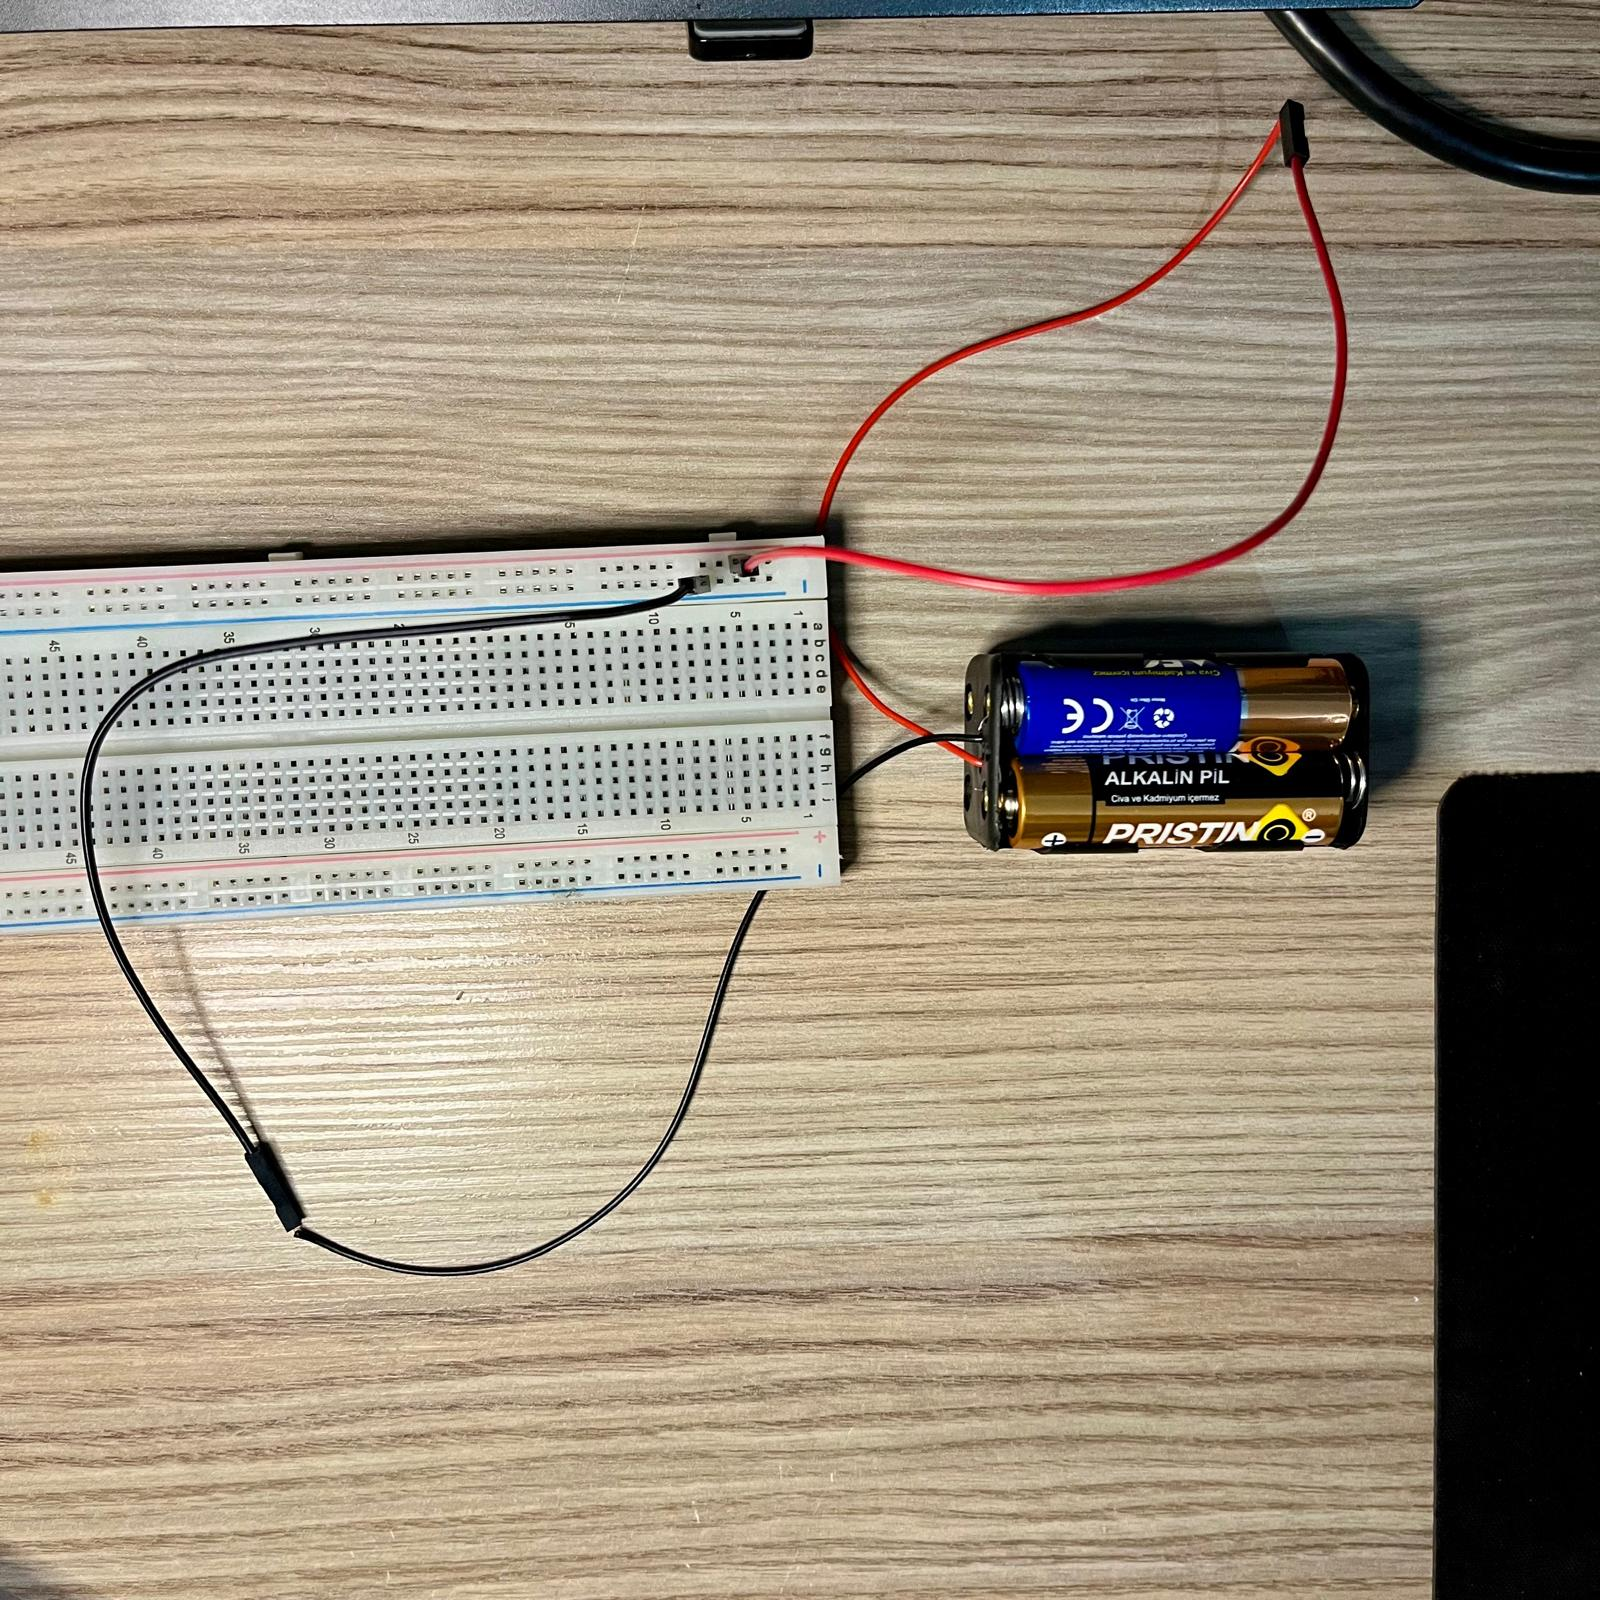
\includegraphics[width=0.42\textwidth]{6v_guc.jpeg}
	\caption{Güç besleme bağlantı şeması}
    \label{fig:guc}
\end{figure}

